
\subsection{Relay attacks}
\begin{description}
    \item[Relay Attack] A relay attack is a form of man-in-the-middle where the
    adversary manipulates the communication by only relaying the verbatim
    messages between two parties.
    \item[Man-In-The-Middle Attack] A man-in-the-middle (MITM) us a form of
    attack, where the adversary provokes or manipulates the communication
    between two parties. Manipulating the communication means relay, withold, or
    insert messages.
\end{description}

\begin{figure}[ht!]
    \centering
    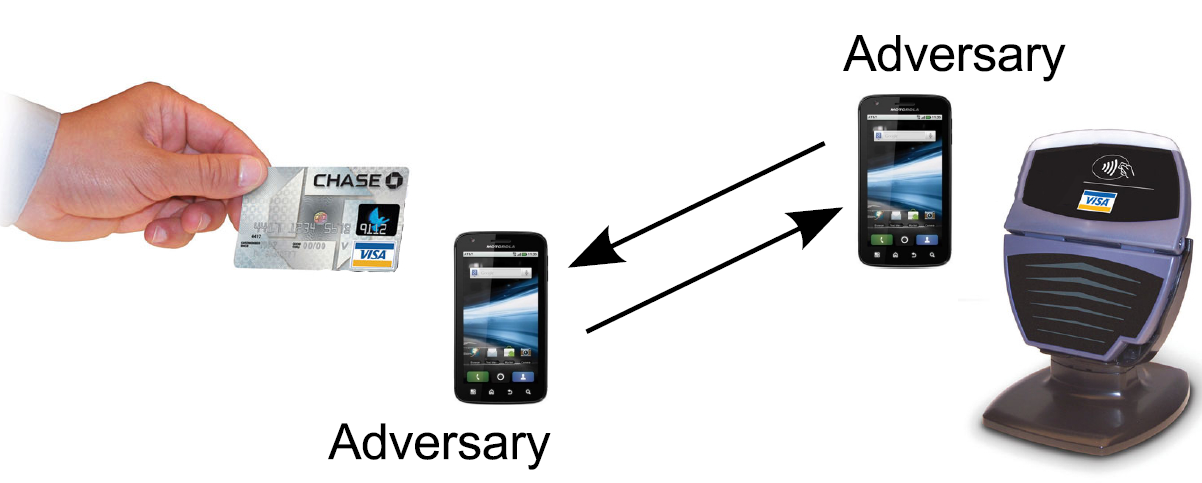
\includegraphics{img/relay-attack}
\end{figure}
\paragraph{Note:} The do-ability of the Relay attack depends on the timer
between the prover and the verifier. Usually the timer is not tight, by default
its 5ms but it can be extend by the prover.


\begin{description}
    \item[Distance Bounding] A distance bounding is a process whereby one party
    assured:
    \begin{itemize}
        \item Of the identity of a second party,
        \item That the latter is present in the neighborhood of the verifying
        party, at some point in the protocol
    \end{itemize}
\end{description}
\paragraph{Note:} Distance bounding protocol does not avoid relay attacks, if
adversary inside the area of coverage.

Measurement of the distance can be done in different ways:
\begin{itemize}
    \item With the GPS
    \item The strength of the received signal  (RSS)
    \item Round Trip Time (RTT)
\end{itemize}

\subsection{Protocol Analysis}
\begin{description}
    \item[Mafia Fraud] A mafia fraud is an attack where an adversary defeats a
    distance bounding protocol using a man-in-the-middle (MITM) between the
    reader and an honest tag located outside the neighborhood.
    \item[Terrorist Fraud] A terrorist fraud is an attack where an adversart
    defeats a distance bounding protocol using a man-in-the-middle (MITM)
    between the reader and dishonest tag located outside of the neighborhood,
    such that the latter actively helps the adversary to maximize her attack
    success probability, without giving to her any advantage for future attacks
    \item[Distance Fraud] Given a distance bounding protocol, a distance fraud
    is an attack where a dishonest and lonely prover purports to be in the
    neighborhood of the verifier.
\end{description}

%%TODO Hancke and Kuhn's Protocol

\subsection{Comparison with Decision Theory}
%%NOT sure if we have seen this
